\section{Application}
\label{sec:application}

\subsection{Network Function}

Network functions~\cite{li2016clicknp}, ClickOS~\cite{martins2014clickos}

Scenarios: Firewall (no packet change), NAT (change a packet field), Tunnel endpoint (add/remove packet header, change length)

Metrics: Latency, throughput

\begin{figure}[htpb]
	\centering
	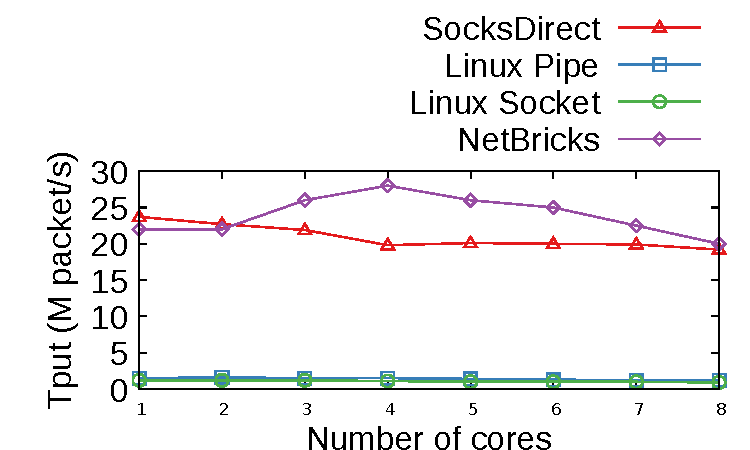
\includegraphics[width=\columnwidth]{eval/microbenchmark/nfv-tun-tput.pdf}
	\caption{Throughput of NFV tunnel}
	\label{fig:eval-tun-tput}
\end{figure}



\subsection{Web Application}

Nginx~\cite{nginx}, Nodejs~\cite{nodejs} and memcached~\cite{memcached}

\begin{itemize}
	\item Figure~\ref{fig:eval-nginx-short}: Many short-lived connections. Nginx $\rightarrow$ Nodejs, Nodejs access memcached once.
	\item Figure~\ref{fig:eval-nginx-multiround}: Each connection, backend interact extensively. (Nodejs access memcached multiple round trips.)
	\item Figure~\ref{fig:eval-nginx-long}: Long connection to download a large in-memory file. (test zero copy)
\end{itemize}

\begin{figure}[htpb]
	\centering                                                         
	\subfloat[Throughput of Simple Short-lived connections]{                    
		%\begin{minipage}{0.4\textwidth}
			\centering
			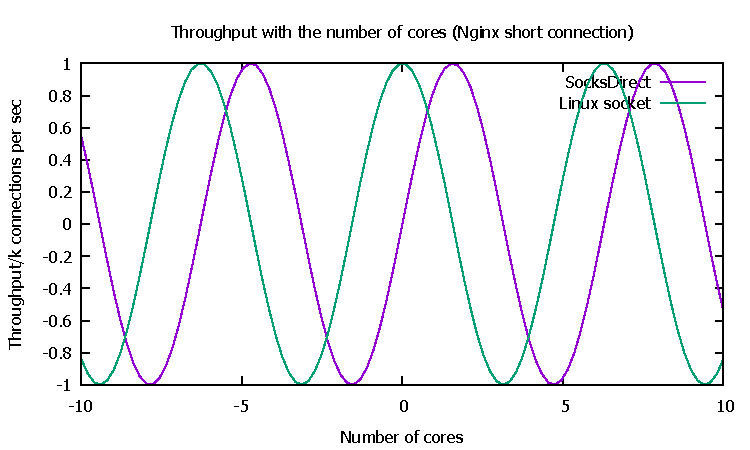
\includegraphics[width=\columnwidth]{eval/microbenchmark/nginx-short-tput.pdf}
			\label{fig:eval-nginx-short}
		%\end{minipage}
		}
	
	\subfloat[Latency of complicated requests]{
		%\begin{minipage}{0.4\textwidth}
			\centering 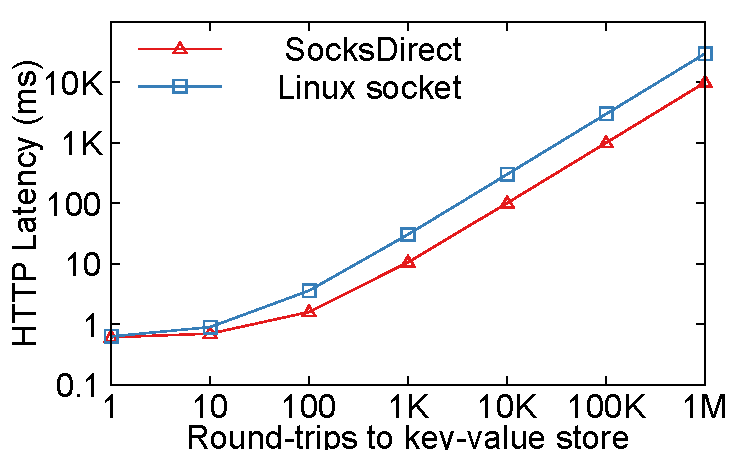
\includegraphics[width=\columnwidth]{eval/microbenchmark/nginx-multiround-tput.pdf}
			\label{fig:eval-nginx-multiround}
		%\end{minipage}
		}

		\subfloat[Transmission throughput of a long-lived connection]{
		%\begin{minipage}{0.4\textwidth}
			\centering 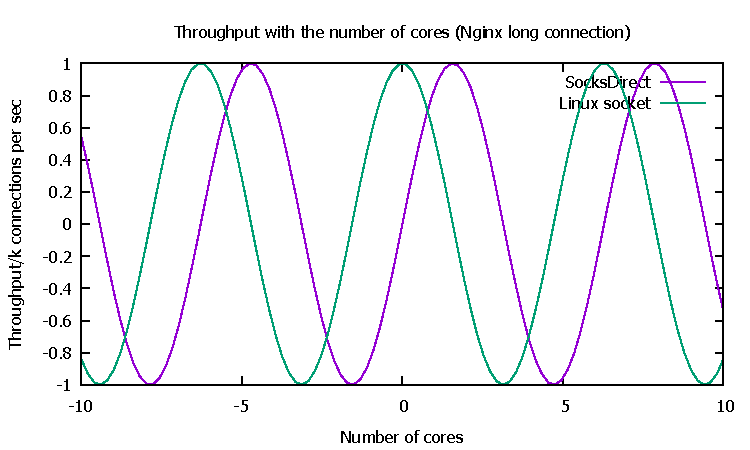
\includegraphics[width=\columnwidth]{eval/microbenchmark/nginx-long-tput.pdf}
			\label{fig:eval-nginx-long}
		%\end{minipage}
		}
		
		\caption{Performance of a web service composed of Nginx, Node.js and memcached.}
		\label{fig:eval-nginx-tput}                                           
\end{figure}


%\subsection{Real-time Stream Processing}

%Apache Flink~\cite{carbone2015apache} (need to turn off durability on disk)

%Scenario: Word Count (distributed system with one source, two mappers and one reducer)

%Metrics: Latency, throughput

%\subsection{Machine Learning}

%Tensorflow~\cite{abadi2016tensorflow}

%Scenario: (Distributed Tensorflow) Parameter server and worker on a same server.

%Metrics: Time per iteration